\documentclass[sigconf,10pt,nonacm]{acmart}

% MobiArch 2026 asks for the ACM template, 10pt, two columns, US Letter.
% The nonacm option removes ACM rights metadata for the submission draft.
\settopmatter{printacmref=false}
\renewcommand\footnotetextcopyrightpermission[1]{}
\pagestyle{plain}

\usepackage{amsmath}
\usepackage{graphicx}
\usepackage{booktabs}
\usepackage{multirow}
\usepackage{subcaption}
\usepackage{siunitx}
\usepackage[ruled,vlined]{algorithm2e}
\usepackage{enumitem}
\usepackage[capitalize]{cleveref}

\setlist{leftmargin=*,itemsep=0.12em,topsep=0.2em}
\sisetup{detect-all}

\title{OrbitLLM: Profile-Anchored Large-Model Scheduling for LEO/NTN Mobile Edge Systems}

\author{Anonymous Author(s)}
\affiliation{%
  \institution{Affiliation}
  \city{City}
  \country{Country}}
\email{email@domain}

\begin{document}
% Auto-generated by orbitllm.plot
\newcommand{\ProfileRows}{%
1.7B & INT4 & 25.4 & 2.4/3787.2 & 2.9\\
3B & INT4 & 22.7 & 5.2/4668.7 & 4.1\\
8B & INT4 & 20.2 & 16.0/7018.6 & 7.7\\
}
\newcommand{\ActionMixRows}{%
All-Downlink & 0.0 & 0.0 & 100.0 & 0.0\\
All-On-Board & 75.8 & 0.0 & 0.0 & 24.2\\
Fixed-Threshold & 40.7 & 34.8 & 24.5 & 0.0\\
\textbf{Heuristic-TVD} & 75.7 & 6.7 & 17.6 & 0.0\\
}
\newcommand{\MainResultRows}{%
All-Downlink & 0.59$\pm$0.01 & 0.0 & 0.0 & 36.1\\
All-On-Board & 0.75$\pm$0.01 & 760.7 & 100.0 & 1.1\\
Fixed-Threshold & 0.85$\pm$0.01 & 355.1 & 64.4 & 6.4\\
\textbf{Heuristic-TVD} & 0.90$\pm$0.01 & 585.2 & 84.9 & 1.0\\
MILP-Bound & 1.00$\pm$0.00 & 576.9 & -- & --\\
}


\begin{abstract}
Emerging 6G non-terrestrial networks (NTNs) make LEO satellites intermittent mobile-edge nodes, but current offloading models still treat workloads as generic bits or CPU cycles. This abstraction is brittle for large language models (LLMs): autoregressive inference has a key--value cache memory wall, and prefill and decode tokens have different energy costs. We present \textbf{OrbitLLM}, a profile-anchored scheduling framework that exposes LLM energy, latency, and memory surfaces to an online LEO/NTN edge scheduler. Rather than treating our host as spacecraft hardware, we profile $1.7$--$8$B Qwen-family models on an RTX 4090 24GB availability anchor and make the profile table replaceable. Given visibility windows, value half-lives, battery budget, downlink capacity, and memory limits, OrbitLLM chooses among full on-board inference, raw downlink, and lightweight pre-screening with partial downlink. A mixed-integer program gives an offline upper bound, while Heuristic-TVD implements a constant-time value-density rule. In 24-hour simulations with 10 random seeds, Heuristic-TVD reaches $0.90\pm0.01$ normalized value, above All-Downlink ($0.59\pm0.01$), All-On-Board ($0.75\pm0.01$), and Fixed-Threshold ($0.85\pm0.01$). Additional network-contact, pre-screen, and hardware-scaling sweeps show that the scheduler adapts its ON/PRE/DOWN action mix as NTN resources and profile costs change.

\end{abstract}

\keywords{LEO/NTN edge computing, large language models, on-board inference, energy-aware offloading, KV cache}

\maketitle

\section{Introduction}
\label{sec:intro}

LEO satellites are becoming part of the mobile Internet architecture rather than isolated space relays. In emerging 6G non-terrestrial networks (NTNs), satellites may serve remote sensors, direct-to-device links, and delay-sensitive mobile services during intermittent contacts. At the same time, sensing pipelines are moving from narrow convolutional models toward large language and vision--language models~\cite{huo2025when,weng2025visionlanguage,mai2024opportunities}. The natural next step is to process high-value observations at the orbital edge instead of always waiting for a ground-station pass.

The scheduling literature is not yet ready for this step. Most satellite-edge offloading formulations model a task by its input bits, CPU cycles, or service delay~\cite{li2025delaycost,zhao2025region,gao2024hierarchical}. That view misses two facts that dominate LLM inference. First, peak memory grows with context through the KV cache; a schedule that ignores this boundary can select an on-board action that simply does not fit. Second, prefill and decode tokens have different energy and throughput behavior because the former is compute-heavy and the latter is memory-bandwidth-heavy~\cite{li2024survey,kim2025oaken}. A scheduler that collapses them into one average cost misprices long generations, exactly the case expected in open-ended Earth-observation reports.

This paper develops OrbitLLM as a workshop-scale scheduling layer for LEO/NTN mobile edge systems. We do not attempt to reproduce a full orbital hardware campaign. Instead, we build a measured LLM cost surface from RTX 4090 availability-anchor profiles and study how such a replaceable profile changes the on-board/downlink decision. Each task has a data size, required model scale, and exponentially decaying value. The policy selects one of three architecture actions: run the model on board, downlink the raw data for ground inference, or run a lightweight semantic pre-screen and downlink only retained evidence.

Our contributions are:
\begin{itemize}
  \item \textbf{LLM-aware cost model.} We expose prefill energy, decode energy, throughput, and peak memory as explicit functions of model scale, quantization, and context length.
  \item \textbf{Energy--value formulation.} We combine the LLM cost surface with orbital visibility windows, battery limits, downlink capacity, and time-decaying task values.
  \item \textbf{Lightweight scheduler.} We give a MILP upper bound and a deployable heuristic, Heuristic-TVD, that greedily maximizes value density while enforcing hard energy and memory feasibility.
  \item \textbf{Reproducible simulation.} We release a Python pipeline that generates task traces, runs baselines, performs network/PRE/hardware sweeps, writes CSV results, and regenerates every plot and table.
\end{itemize}

\section{Related Work}
\label{sec:related}

\subsection{NTN and Satellite Edge Computing}
LEO systems are increasingly studied as part of the mobile/NTN edge rather than only as bent-pipe relays. Recent work optimizes delay--cost trade-offs for emergency tasks~\cite{li2025delaycost}, adaptive offloading across heterogeneous constellations~\cite{zhao2025region}, hierarchical resource allocation~\cite{gao2024hierarchical}, and deep-RL user association or service migration~\cite{zhang2024dynamic,wu2024task}. These formulations are valuable, but their workload model is typically a divisible amount of bits or CPU cycles. OrbitLLM keeps the orbital visibility and resource-allocation view, but replaces the generic compute abstraction with LLM-specific memory and token-energy constraints.

\subsection{Mobile Edge AI and Pre-Screening}
Space-AI systems have shown that compact neural models can run near the sensor. Reviews summarize hardware and software support for satellite inference~\cite{diana2024review,lonard2026fpgaenabled}, while systems such as Kodan show the benefit of selecting valuable data before expensive processing or downlink~\cite{denby2023kodan}. Remote-sensing foundation models and VLM datasets are rapidly improving the capability side~\cite{huo2025when,weng2025visionlanguage,wang2024skyscript}. OrbitLLM treats pre-screening as an architecture action: a lightweight module retains semantic evidence under a configurable bit-retention and utility-retention curve.

\subsection{Efficient LLM Inference}
Efficient LLM inference provides the mechanisms that make on-board deployment plausible: quantization, KV-cache compression, small language models, and memory-aware serving~\cite{zhou2024survey,bai2024beyond,wang2024comprehensive}. KV-cache management is especially relevant because it determines whether long-context inference fits a constrained accelerator~\cite{li2024survey,kim2025oaken,alizadeh2024flash}. OrbitLLM does not propose a new compression method; it treats the measured or parameterized effect of those methods as the cost surface used by the scheduler.

\section{System Model and Problem Formulation}
\label{sec:system}

\subsection{Scenario}
We consider one LEO/NTN edge node equipped with a sensor-facing task queue, a constrained accelerator, and an intermittent downlink. As shown in \Cref{fig:arch}, tasks enter an on-board queue. A replaceable LLM profile supplies energy, latency, and memory costs; an orbital contact schedule supplies ground-station windows; the scheduler selects an action for each task.

\begin{figure}[tb]
  \centering
  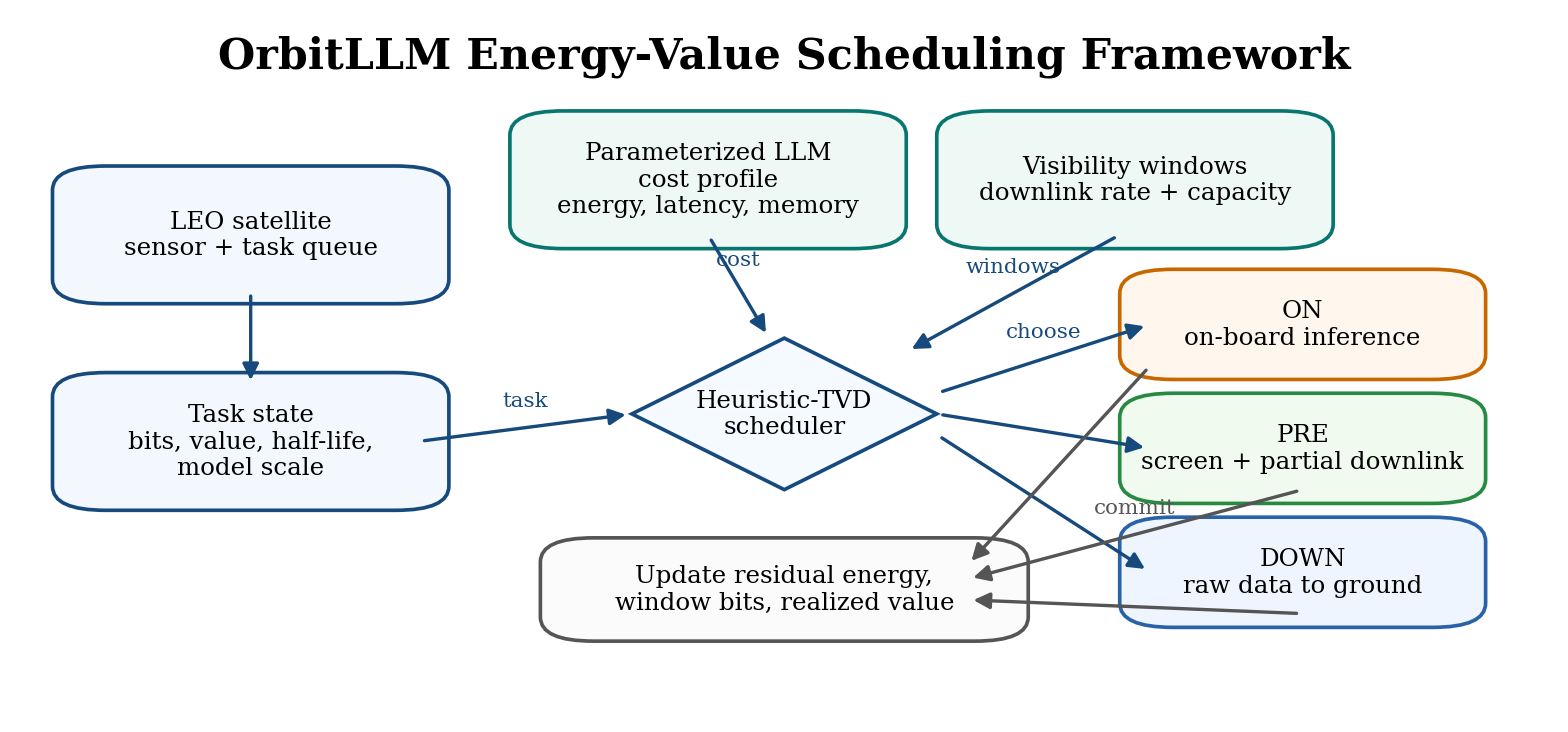
\includegraphics[width=\columnwidth]{figures/architecture.png}
  \caption{OrbitLLM architecture. A profile of LLM inference costs and a visibility-window timeline feed an online energy--value scheduler that chooses on-board inference, direct downlink, or pre-screening with partial downlink.}
  \label{fig:arch}
\end{figure}

\subsection{Visibility and Tasks}
The horizon is discretized into time slots $t=1,\ldots,T$ of duration $\Delta$. The orbital schedule gives a visibility indicator $v_t$ and rate $r_t$ when $v_t=1$. For a visibility window $w$, the available downlink capacity is
\begin{equation}
B_w=\sum_{t\in w} r_t\Delta .
\label{eq:bw}
\end{equation}
Task $i$ arrives at time $a_i$ and is described by $(d_i,s_i,V_i^0,\tau_i,n_i^p,n_i^d)$: raw bits, required model scale, immediate value, value half-life, prefill tokens, and decode tokens. If completed at time $c_i$, the realized value is
\begin{equation}
V_i(c_i)=V_i^0\exp\!\left(-\frac{c_i-a_i}{\tau_i}\right), \qquad c_i\ge a_i .
\label{eq:value}
\end{equation}
Small $\tau_i$ models time-critical observations such as wildfire onset; large $\tau_i$ models archival mapping.

\subsection{Actions and LLM Costs}
The scheduler chooses $x_i\in\{\textsc{on},\textsc{down},\textsc{pre}\}$. \textsc{on} runs the full model on board; \textsc{down} transmits raw data; \textsc{pre} is a lightweight semantic compression action inspired by value-aware data selection~\cite{denby2023kodan}. It can be implemented by an ROI selector, confidence-gated detector, or small encoder that emits metadata plus selected patches. We model it by a retained-bit ratio $\rho_i$ and a utility-retention factor $\eta_i$: it transmits $\rho_i d_i$ bits and realizes $\eta_i V_i(c_i)$. These parameters are not hidden constants; \Cref{sec:exp} sweeps them to show when PRE is useful. For model scale $s_i$, quantization $q$, and context $n_i^p+n_i^d$, the profile gives prefill energy $e^p$, decode energy $e^d$, throughput, and peak memory. Full on-board energy is
\begin{equation}
E_i^{\textsc{on}}=e^p_{s_i,q}n_i^p+e^d_{s_i,q}n_i^d .
\label{eq:eon}
\end{equation}
The pre-screen action uses a configurable fraction of this energy and memory and is evaluated across multiple $\rho_i,\eta_i$ regimes.

\subsection{Optimization Problem}
The objective is to maximize cumulative value subject to battery, downlink, and memory feasibility:
\begin{align}
\max_{\{x_i,\rho_i\}}\quad & \sum_i V_i(c_i(x_i)) \label{eq:obj}\\
\text{s.t.}\quad
& \sum_{i:x_i=\textsc{on}}E_i^{\textsc{on}}+\sum_{i:x_i=\textsc{pre}}E_i^{\textsc{pre}}\le E^{\max}, \label{eq:c-energy}\\
& \sum_{i\in w} b_i(x_i)\le B_w,\quad \forall w, \label{eq:c-bw}\\
& \mathrm{peakmem}(s_i,q,n_i^p+n_i^d)\le M^{\max}. \label{eq:c-mem}
\end{align}
Here $b_i(\textsc{down})=d_i$, $b_i(\textsc{pre})=\rho_i d_i$, and $b_i(\textsc{on})=0$; PRE values are multiplied by $\eta_i$. Even with known arrivals this contains a multiple-choice knapsack problem; the MILP in \Cref{sec:policy} is therefore an offline upper bound rather than an on-board algorithm.

\section{Parameterized LLM Cost Model}
\label{sec:bench}

\subsection{Profile Interface}
OrbitLLM uses a profile table rather than a generic CPU-cycle cost. Each row contains model name, scale, quantization, context length, prefill tokens, decode tokens, prefill joules/token, decode joules/token, decode throughput, peak memory, and GPU power. We generated this table on a remote RTX 4090 24GB host using local copies of \texttt{Qwen3-1.7B}, \texttt{Qwen2.5-3B-Instruct}, and \texttt{Qwen3-8B}. The benchmark covers FP16, INT8, and INT4 inference at 1024, 2048, and 4096-token contexts with three runs per point; repeated runs are averaged before simulation. Replacing \texttt{results/profile\_anchor.csv} with another measured CSV automatically regenerates all scheduling results.

\subsection{Energy and Memory Surfaces}
\Cref{fig:energy} shows the measured separation between prefill and decode energy. The distinction matters because a long generation consumes more energy than a single averaged token coefficient would predict. \Cref{fig:memheat} shows peak memory over model scale and context length. This surface is used as a hard feasibility check in \cref{eq:c-mem}; if a task exceeds the memory ceiling, it cannot be assigned to \textsc{on}.

\begin{figure}[tb]
  \centering
  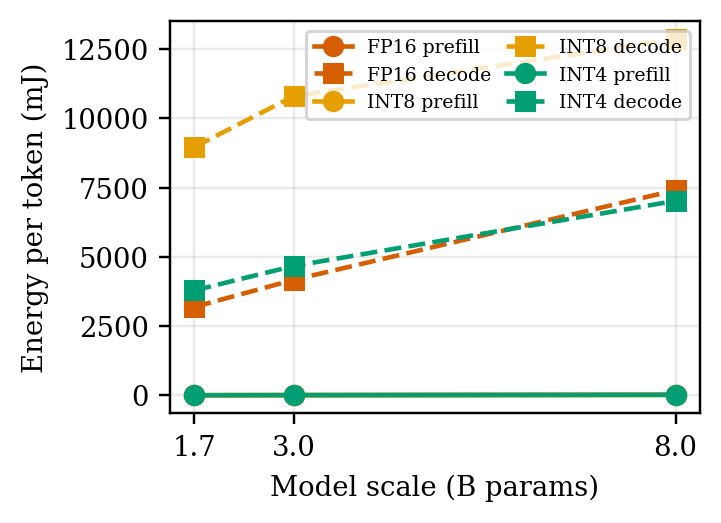
\includegraphics[width=\columnwidth]{figures/energy_per_token.png}
  \caption{Prefill and decode energy per token at 2048-token context. The scheduler indexes this surface when computing \cref{eq:eon}.}
  \label{fig:energy}
\end{figure}

\begin{figure}[tb]
  \centering
  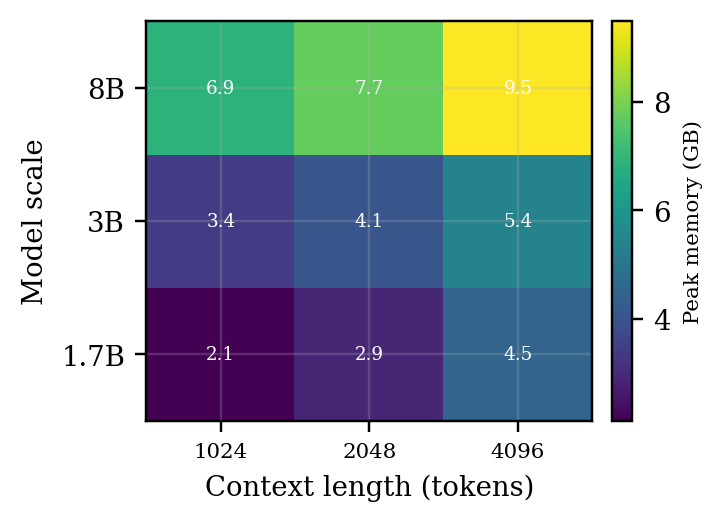
\includegraphics[width=\columnwidth]{figures/mem_heatmap.png}
  \caption{Peak memory for INT4 inference as a function of model scale and context length. The simulation uses a 16 GB on-board memory ceiling; all measured INT4 anchors fit below it.}
  \label{fig:memheat}
\end{figure}

\begin{table}[tb]
\centering
\caption{INT4 profile rows used by the reported simulation at 2048-token context. Energy is prefill/decode mJ per token, averaged over three runs.}
\label{tab:profile}
\small
\begin{tabular}{llccc}
\toprule
Model & Quant. & Tok/s & Energy/tok & Peak mem \\
\midrule
\ProfileRows
\bottomrule
\end{tabular}
\end{table}

\subsection{Why Parameterization Helps}
The purpose of this profile is not to claim flight-hardware performance. It is to make the scheduling assumption explicit and replaceable. Existing offloading models hide LLM behavior behind a scalar compute cost; OrbitLLM exposes the quantities that determine feasibility and value: memory fit, on-board latency, and token-level energy. The measured bitsandbytes INT8 path is not universally better than FP16 on this host, which reinforces the need to use hardware-specific profile rows rather than assumed quantization multipliers.

\section{Scheduling Algorithms}
\label{sec:policy}

\subsection{MILP Upper Bound}
With full knowledge of arrivals and windows, \cref{eq:obj}--\cref{eq:c-mem} can be solved as a mixed-integer linear program. We introduce binary variables $y_i^a$ for action $a\in\{\textsc{on},\textsc{down},\textsc{pre}\}$ and impose $\sum_a y_i^a=1$. The energy constraint is global, the bandwidth constraint is per visibility window, and infeasible memory choices receive zero eligibility. The MILP is solved only offline on the ground and gives an upper bound for causal policies.

\subsection{Heuristic-TVD}
The deployable policy is a constant-time value-density rule. For every arriving task, it computes the feasible completion time and realized value for each action. Let $V_i(a)$ be the realized value of action $a$ and let $V_i(\textsc{down})$ be the direct-downlink reference. We score each feasible action by
\begin{equation}
\mathrm{TVD}_i(a)=
\frac{V_i(a)+\beta\max(0,V_i(a)-V_i(\textsc{down}))}
{\epsilon+\lambda_E E_i(a)/\max(E_{\mathrm{res}},1)+\lambda_B b_i(a)/d_i}.
\label{eq:tvd}
\end{equation}
The numerator rewards both absolute value and value recovered relative to waiting for downlink; the denominator penalizes scarce energy and bandwidth. Actions violating memory or residual energy are removed before scoring.

\begin{algorithm}[tb]
\small
\caption{Heuristic-TVD Online Scheduling}
\label{alg:policy}
\KwIn{tasks, visibility windows, energy budget $E^{\max}$, memory ceiling $M^{\max}$, LLM profile $\Theta$}
\KwOut{action $x_i$ for each task}
$E_{\mathrm{res}}\leftarrow E^{\max}$; initialize downlink queue\;
\For{each task $i$ in arrival order}{
  read $(e^p,e^d,\mathrm{tok/s},\mathrm{peakmem})$ from $\Theta$\;
  enumerate $a\in\{\textsc{on},\textsc{down},\textsc{pre}\}$\;
  remove actions that exceed $E_{\mathrm{res}}$ or $M^{\max}$\;
  estimate completion time, value, energy, and bits for each remaining action\;
  $x_i\leftarrow\arg\max_a \mathrm{TVD}_i(a)$\;
  commit compute energy and downlink bits for $x_i$\;
}
\end{algorithm}

\subsection{Baselines}
We compare against \textsc{All-Downlink}, which queues every raw observation for ground inference; \textsc{All-On-Board}, which runs on board until energy or memory prevents it; and \textsc{Fixed-Threshold}, which uses a static value threshold to decide whether to process or pre-screen on board. These baselines isolate the benefit of using time decay, LLM cost, and residual resources jointly.

\section{Evaluation}
\label{sec:exp}

\subsection{Setup}
The simulator runs a 24-hour horizon with 10 random seeds. Unless otherwise stated, traces use a 90-minute orbit, a 10-minute contact window, and a 35 Mbps downlink. Each trace contains 260 heterogeneous tasks with model scales in $\{1.7,3,8\}$B, log-normal data sizes, urgent and routine half-lives, and configured prefill/decode token counts. The on-board compute-energy budget is 150 kJ and the memory ceiling is 16 GB. The default PRE module uses 18\% of full on-board inference energy/latency, retains 32\% of raw bits, and keeps 94\% of task utility; \Cref{fig:pre} sweeps these assumptions. All numbers and plots are regenerated from CSV files produced on the remote RTX 4090 server.

\subsection{Main Results}
\Cref{fig:value} and \Cref{tab:main} compare Heuristic-TVD with three baselines and the MILP upper bound. All-Downlink loses value because urgent tasks wait for contacts. All-On-Board has low latency but exhausts energy and drops tasks. Fixed-Threshold uses task value but cannot jointly adapt to residual energy, bandwidth, and model memory. Heuristic-TVD reaches $0.90\pm0.01$ normalized value, above All-Downlink ($0.59\pm0.01$), All-On-Board ($0.75\pm0.01$), and Fixed-Threshold ($0.85\pm0.01$), while reporting zero OOM and zero energy violations.

\begin{figure}[tb]
  \centering
  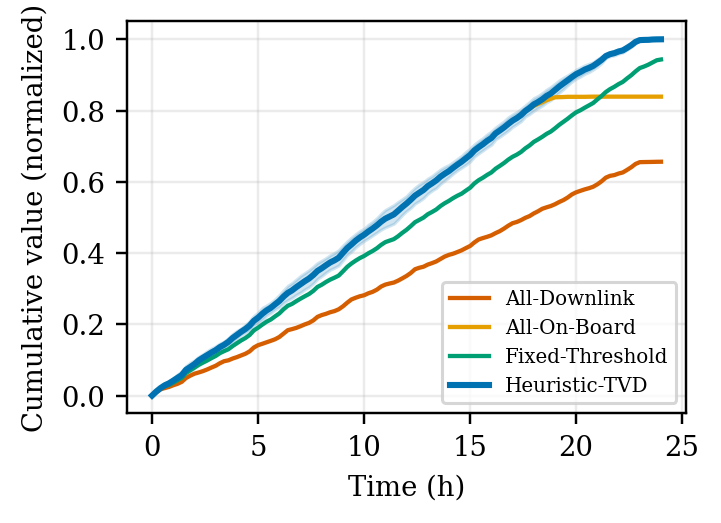
\includegraphics[width=\columnwidth]{figures/value_curve.png}
  \caption{Cumulative realized value over 24 hours. Heuristic-TVD preserves energy for later high-value tasks while still serving urgent tasks early.}
  \label{fig:value}
\end{figure}

\begin{table}[tb]
\centering
\caption{Main 24-hour results over 10 seeds. Value is normalized by the MILP bound; bandwidth saving is relative to All-Downlink.}
\label{tab:main}
\scriptsize
\begin{tabular}{lcccc}
\toprule
Method & Value$\uparrow$ & J/task$\downarrow$ & BW save$\uparrow$ & Lat. med.$\downarrow$\\
\midrule
\MainResultRows
\bottomrule
\end{tabular}
\end{table}

\begin{table}[tb]
\centering
\caption{Action mix in the main experiment. PRE is selected only when partial semantic transfer is more valuable than raw downlink under residual resources.}
\label{tab:mix}
\scriptsize
\begin{tabular}{lcccc}
\toprule
Method & ON & PRE & DOWN & DROP\\
\midrule
\ActionMixRows
\bottomrule
\end{tabular}
\end{table}

\subsection{NTN Contact Sensitivity}
\Cref{fig:network} varies the network regime. At low downlink rates, Heuristic-TVD preserves value by avoiding raw transfers and using ON/PRE for urgent tasks. As contact windows expand, the action mix shifts smoothly because the value-density denominator accounts for both residual energy and bandwidth. This is the key MobiArch point: the policy is an architecture-level adaptation layer, not a single fixed offloading threshold.

\begin{figure}[tb]
  \centering
  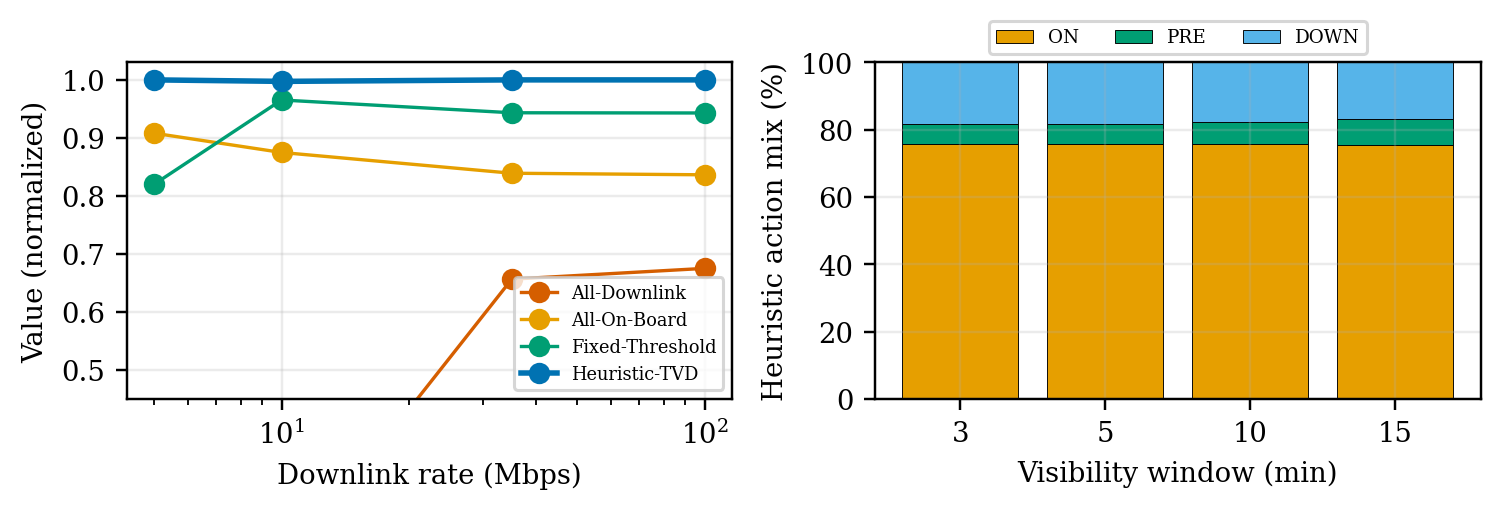
\includegraphics[width=\columnwidth]{figures/network_sensitivity.png}
  \caption{Network/contact sensitivity. Left: value across downlink rates. Right: Heuristic-TVD action mix as visibility windows change.}
  \label{fig:network}
\end{figure}

\subsection{PRE and Hardware Sensitivity}
\Cref{fig:pre} sweeps PRE retained-bit ratio $\rho$ and utility-retention model $\eta(\rho)$. PRE is most useful in the middle regime: aggressive filtering saves bandwidth but can lose value, while large $\rho$ approaches raw downlink. This turns PRE from a black-box assumption into an explicit design space.

\begin{figure}[tb]
  \centering
  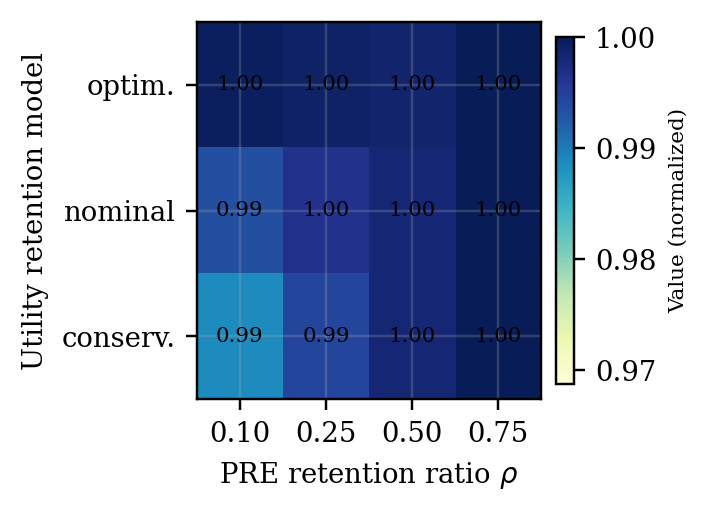
\includegraphics[width=\columnwidth]{figures/pre_sensitivity.png}
  \caption{PRE sensitivity over retained bits and utility-retention regimes. Values are normalized against the best PRE/no-PRE choice for the same seed and setting.}
  \label{fig:pre}
\end{figure}

\Cref{fig:hardware} scales the measured 4090 energy and latency profile by $0.5$--$4\times$. Faster profiles choose full on-board inference; constrained profiles shift toward PRE and DOWN while preserving feasibility. Thus the framework does not rely on the 4090 as target hardware: it consumes a replaceable cost surface.

\begin{figure}[tb]
  \centering
  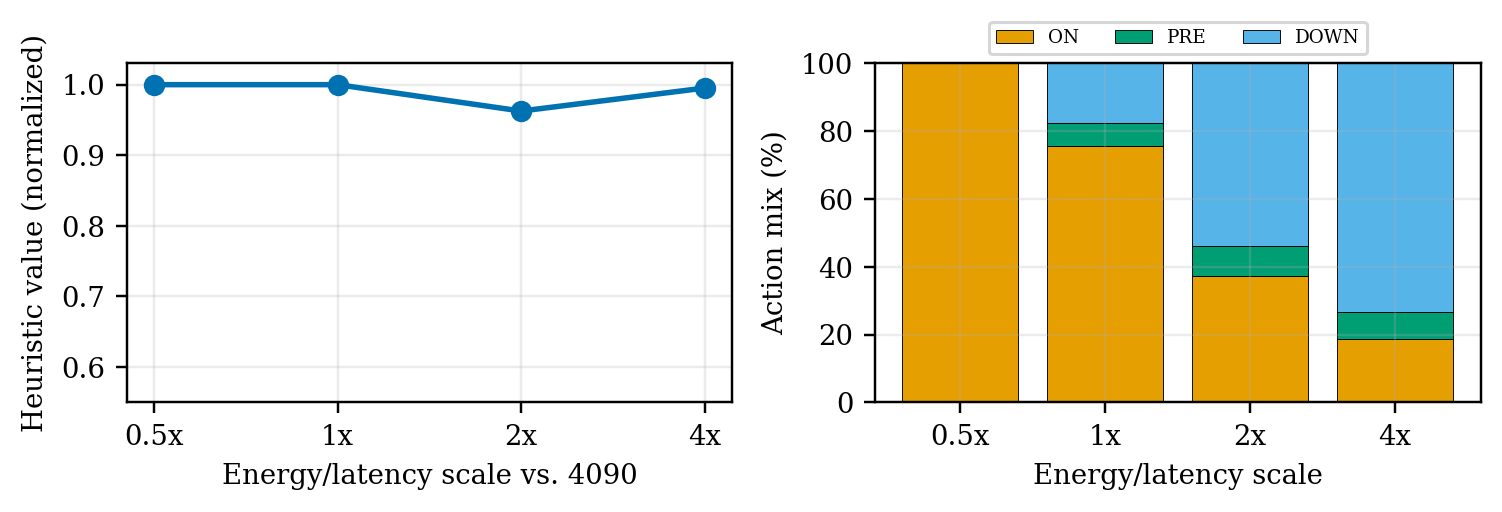
\includegraphics[width=\columnwidth]{figures/hardware_sensitivity.png}
  \caption{Hardware-profile scaling. Heuristic-TVD changes its action mix as the measured profile is scaled from faster accelerators to constrained edge devices.}
  \label{fig:hardware}
\end{figure}

\section{Discussion and Limitations}
\label{sec:discuss}

OrbitLLM's main point is architectural: LEO/NTN mobile-edge schedulers need a runtime interface that exposes the quantities binding large-model inference. Bits and CPU cycles are insufficient when memory fit depends on KV cache length and energy depends on the prefill/decode mix. Making these quantities explicit also makes the framework reproducible: changing hardware, quantization, or model family only changes the profile CSV, not the optimizer or simulator.

The most important limitation is that the reported numbers are RTX 4090 availability-anchor measurements, not spacecraft accelerator measurements. The hardware-scaling experiment is intended to test sensitivity to this choice, not to validate a particular on-orbit device. Radiation effects, spacecraft integration, accuracy changes under quantization, and detailed power replenishment are outside the scope of this workshop version.

PRE is also an abstraction rather than a single deployed vision module. We model it as lightweight semantic compression with retained-bit and utility-retention parameters, then sweep those parameters to expose when the action helps. A deployment would calibrate this curve with a concrete ROI selector, detector, or small vision-language encoder. Finally, our 24-hour traces are generated by a discrete-event simulator; future work should add real contact traces, multi-satellite interactions, and measured profiles from flight-relevant edge accelerators.

\section{Conclusion}
\label{sec:conclusion}
We presented OrbitLLM, a profile-anchored scheduling framework for large-model inference in LEO/NTN mobile edge systems. By turning LLM-specific inference behavior into a replaceable cost profile, the framework avoids the generic bits/cycles abstraction used by conventional offloading models. A simple value-density heuristic, calibrated against a MILP upper bound, outperforms All-Downlink, All-On-Board, and fixed-threshold baselines while respecting energy and memory constraints. Network, PRE, and hardware-scaling sweeps show how the ON/PRE/DOWN action mix adapts as mobile-edge resources change.

\section*{Reproducibility Statement}
The artifact contains the benchmark CLI, simulator, MILP bound, plotting scripts, configuration file, generated CSV results, and LaTeX table macros. The code and results are available at \url{https://github.com/1740919441a/OrbitLLM}. Running \texttt{python -m orbitllm.cli simulate} followed by \texttt{python -m orbitllm.cli plot} regenerates the reported tables and figures.


\bibliographystyle{ACM-Reference-Format}
{\footnotesize
\bibliography{refs}
}

\end{document}
